\documentclass[11pt]{book} 
\usepackage{graphicx}
             % Book class in 11 points
\parindent0pt  \parskip10pt             % make block paragraphs
\raggedright                            % do not right justify

\title{\bf Open Calculus}    % Supply information
\author{Editor-in-chief: Adam Cross}   
          %   for the title page.
\date{\today}                           %   Use current date. 

% Note that book class by default is formatted to be printed back-to-back.
\begin{document}                        % End of preamble, start of text.
\frontmatter                            % only in book class (roman page #s)
\maketitle                              % Print title page.
\tableofcontents                        % Print table of contents
\mainmatter                             % only in book class (arabic page #s)

\part{A Part Heading}                   % Print a "part" heading



\chapter{Limits}     


\section{Exercises}

\begin{enumerate}

\item
Refer to the graphs.

\begin{center}
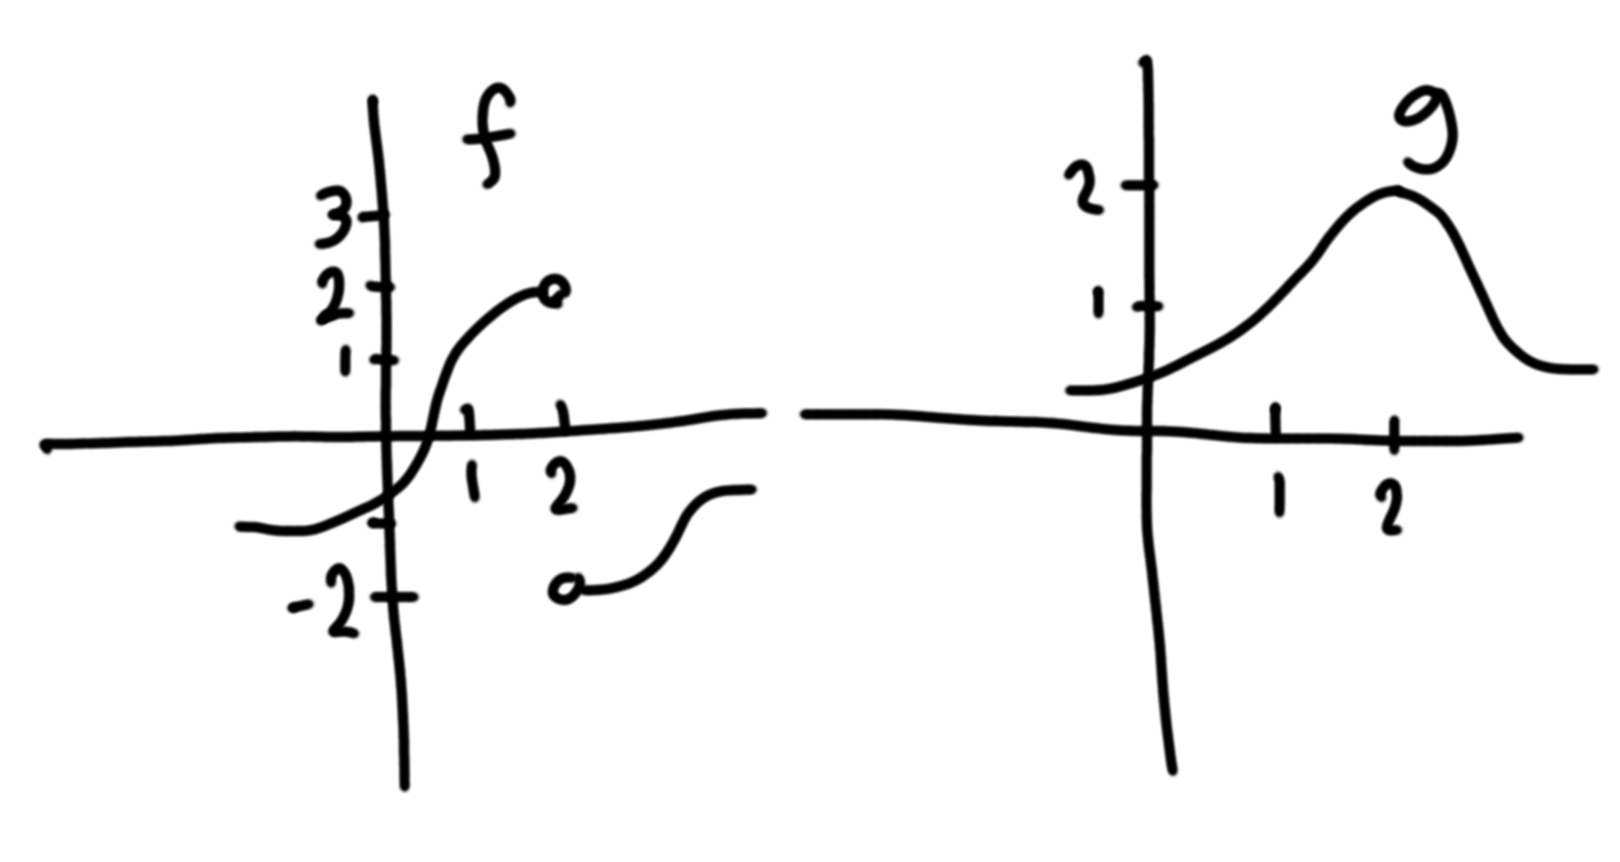
\includegraphics[width=4in]{limitExerciseImage1.png}
\end{center}

What is $\lim_{x\to 2} f(g(x))$?  What is $\lim_{x\to 2} g(f(x))$?


\end{enumerate}




\chapter{Derivatives}  


\chapter{Integrals}  



\end{document}                         